The best networks found among those examined in all set of experiments are the ``CLD'', ``CMCML'' and ``CMCMLL''. They have similar training times and final accuracy results. Their accuracy curves are shown in figure \ref{fig:bestnets}.

\begin{figure}[htb!]
\centering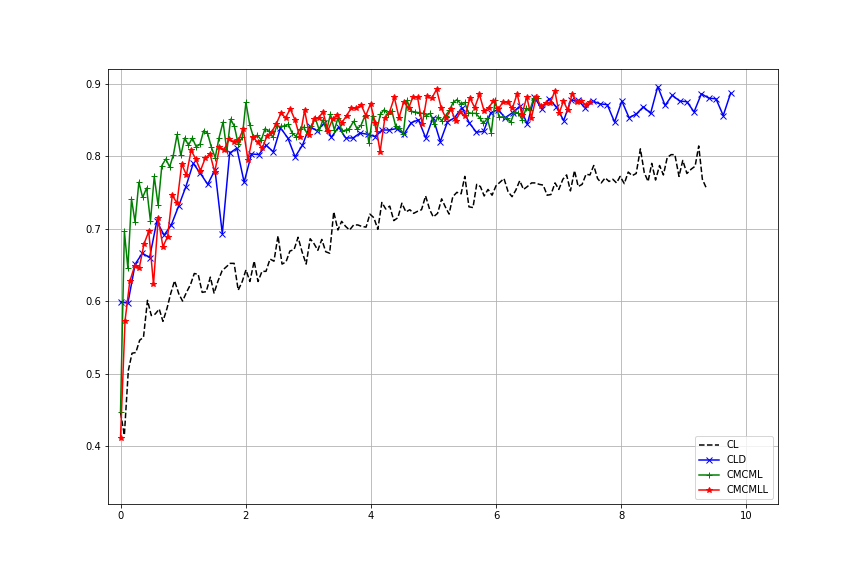
\includegraphics[width=0.50\textwidth]{content/CL-CLD-CMCML-CMCMLL.png}
\caption[Best networks]{\label{fig:bestnets}Three networks with best accuracy - validation accuracy vs. time(minutes)}
\end{figure}

While a simple feedforward network worked well to classify the beginning of a file, there are better options to classify a block sample taken from the middle of the file.

The convolutional and LSTM layers worked well together, better than either one in isolation.

Table \ref{tab:carvinglayers} specify the number of output units in each layer of the networks used in the experiments. For the networks with two convolutional layers, those layers are connected together before the LSTM layer. For the convolutional layers, the input number indicates the size of the receptive field. 
\begin{table*}[!ht]
    \centering
    \caption{Experiments layers}
    \label{tab:carvinglayers}
\begin{tabular}{r|r|r|r|r|r|r}

       & \multicolumn{4}{|c|}{}                         &        & Fully           \\     
       & \multicolumn{4}{|c|}{Convolutional}            & LSTM   &       connected \\ \hline
Name   & Input         & Stride & Output & Pooling size & Output & Output          \\ \hline\hline

D      &               &        &        &              &        & 3               \\ \hline
LD     &               &        &        &              & 32     & 3               \\ \hline
CL     & 32            & 32     & 3      &              & 3      &                 \\ \hline
\hline
CLL    & 32            & 32     & 32     &              & 64     &                 \\       
       &               &        &        &              & 3      &                 \\ \hline
CML    & 32            & 32     & 32     & 2            & 3      &                 \\ \hline
CLD    & 16            & 16     & 256    &              & 128    & 3               \\ \hline
\hline
CM     & 32            & 1      & 3      & 481          &        &                 \\ \hline
CCM    & 32            & 1      & 3      &              &        &                 \\       
       & 2             & 2      & 3      & 240          &        &                 \\ \hline
CD     & 64            & 8      & 64     &              &        & 3               \\ \hline
\hline
CCL    & 8             & 8      & 128    &              & 3      &                 \\       
       & 8             & 8      & 64     &              &        &                 \\ \hline
CCLL   & 8             & 8      & 128    &              & 64     &                 \\       
       & 8             & 8      & 64     &              & 3      &                 \\ \hline

CMCML  & 8             & 8      & 128    & 2            & 3      &                 \\       
       & 8             & 8      & 64     & 2            &        &                 \\ \hline
CMCMLL & 8             & 8      & 128    & 2            & 64     &                 \\       
       & 8             & 8      & 64     & 2            & 3      &                 \\ \hline

\end{tabular}
\end{table*}

The fact that it was possible to distinguish between JPG and PNG file blocks shows the potential of neural networks to perform data carving, as this filetypes have compression and therefore should present few recognizable structures. The PDF file format introduces another type of challenge, as it can enclose the other two filetypes. 